\section{Pedestrian Dead Reckoning}

The \gls{pdr} method is described in \cite{HybridPositioningPaper}. \gls{pdr} tracking is based on step detection algorithms, step length estimations $l_t$ and heading measurements $\theta_t$, all used to solve the problem defined in \textbf{\autoref{eq:pdr_x}} and \textbf{\autoref{eq:pdr_y}}.

\begin{equation} \label{eq:pdr_x}
    x_t = x_{t - 1} + l_t\cos(\theta_t)
\end{equation}

\begin{equation} \label{eq:pdr_y}
    y_t = y_{t - 1} + l_t\sin(\theta_t)
\end{equation}

\begin{figure}[H] \label{fig:pdr}
    \centering
    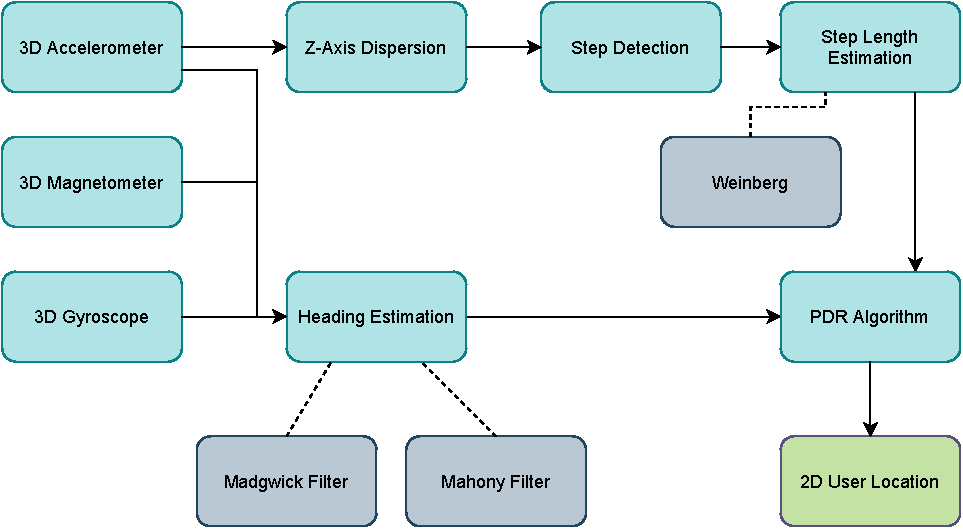
\includegraphics[scale=0.8]{Images/Experiments/pdr.pdf}
    \caption{Caption}
\end{figure}

% Tag elementer fra filen geometry_based.tex fra 1.Problem_analysis til forklaring af PDR.

%https://link.springer.com/article/10.1186/1687-6180-2014-65

%Fast AHRS Filter for Accelerometer, Magnetometer,and Gyroscope Combination with Separated Sensor Corrections

%https://www.researchgate.net/profile/Pasquale-Cirillo-3/publication/303738116_A_comparison_of_multisensor_attitude_estimation_algorithms/links/5750181208aeb753e7b4a0c0/A-comparison-of-multisensor-attitude-estimation-algorithms.pdf

%http://www.cs.ndsu.nodak.edu/~siludwig/Publish/papers/SPIE20181.pdf

%https://core.ac.uk/download/pdf/31017028.pdf

\subsection{Step Detection}

The general idea of step detection of a pedestrian with a smartphone is by measuring the accelerometer sensor, and observe the increases and decreases in the acceleration pattern\cite{HybridPositioningPaper}. We have chosen to follow the algorithm proposed in \cite{peakdetection}. 

The algorithm is based on the principle of dispersion, which is the extent to which a distribution is stretched or squeezed. %https://en.wikipedia.org/wiki/Statistical_dispersion#cite_note-1

In this case, the algorithm will return a signal value if a new datapoint is a specific amount of deviations away from a moving mean. This amount of deviations is also called the z-score. The algorithm creates a seperate moving mean and deviation, and signals can therefore not corrupt the threshold. The algorithm takes 3 inputs: lag, threshold and influence. Lag determines how much the input data is to be smoothened. Therefore, low lag values result in the algorithm being quicker at adapting to the input data. Since the input data for step detection vary a lot, the lag value will be low. The threshold is the z-score at which the algorithm will return a signal. Lastly, the influence is the impact of new signals on the mean and deviation. The influence can be between 0 and 1. If 0 is chosen as the influence, signals would be completely ignored for recalculation of a new threshold. This choice would assume stationarity, meaning that the statistical properties of a process, such as the mean, variance and the structure of the autocorrelation, do not change over time. In our case, we are working with data from walking people in a shopping mall, and since random walking is not a stationary process, we will use 1 as our influence. 

+ lag 
+ threshold


%https://stats.stackexchange.com/questions/246357/why-is-a-random-walk-not-a-stationary-process

%https://www.itl.nist.gov/div898/handbook/pmc/section4/pmc442.htm


%

%https://stackoverflow.com/questions/22583391/peak-signal-detection-in-realtime-timeseries-data/22640362

\subsection{Step Length Estimation}

For step length estimation, there exists two methods: static and dynamic. The static method assumes a person is walking at a constant velocity, whereas the dynamic method makes use of an accelerator for dynamic estimation. Weinberg is one method for dynamic step length estimation, and we have chosen to use the Weinberg method because of its low error compared to other methods \cite{HybridPositioningPaper}.

The Weinberg method is defined as in \textbf{\autoref{eq:weinberg}} \cite{weinberg}.

\begin{equation} \label{eq:weinberg}
    l = k \sqrt[4]{a_{LPF, peak} - a_{LPF, valley}}
\end{equation}

In \textbf{\autoref{eq:weinberg}}, $k$ is a constant factor, for example, $0.5$, $a_{LPF, peak}$ is the maximum acceleration in the z-axis and $a_{LPF, valley}$ is the minimum acceleration. 

\subsection{Heading Estimation}
Heading estimation is accomplished using \gls{ahrs}. \gls{ahrs} is a Python toolkit for estimation attitude containing several functions and utilities for the attitude estimation\cite{ahrs} and \cite{FastAHRS}. According to \cite{MultisensorComparison}, Madgwick and Mahony perform best in comparison to other alternative algorithms, both of which are provided by \gls{ahrs}. Both algorithms compute a set of quaternions, described in \textbf{\autoref{sec:quaternion}}, given a set of acceleration data and gyroscope data, from which a heading can be computed.

\subsection{Quaternions} \label{sec:quaternion}